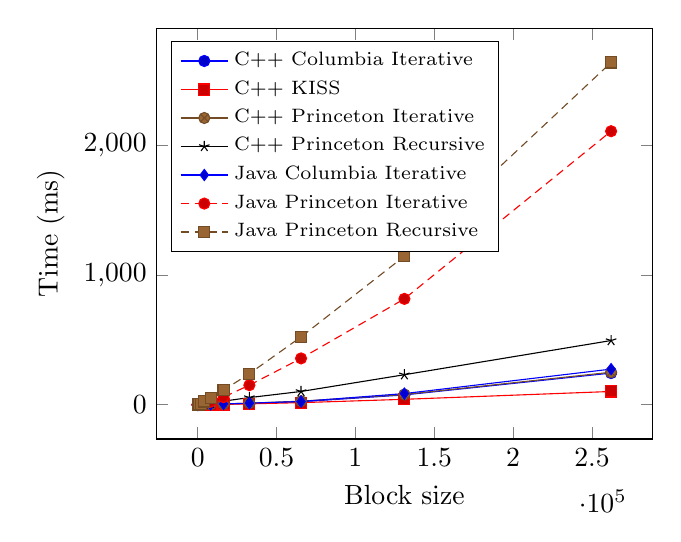
\begin{tikzpicture}
\begin{axis}[xlabel={Block size},ylabel={Time (ms)},width=0.65\linewidth,legend pos=north west,scaled y ticks = false,legend cell align=left,legend style={font=\scriptsize}]
\addplot coordinates {
(16, 0.0072)
(32, 0.0086)
(64, 0.0083)
(128, 0.0115)
(256, 0.0200)
(512, 0.0366)
(1024, 0.0773)
(2048, 0.2604)
(4096, 0.7974)
(8192, 1.9326)
(16384, 4.2789)
(32768, 9.9388)
(65536, 23.1031)
(131072, 75.4942)
(262144, 243.8496)
};
\addplot coordinates {
(16, 0.0056)
(32, 0.0069)
(64, 0.0079)
(128, 0.0131)
(256, 0.0182)
(512, 0.0461)
(1024, 0.0992)
(2048, 0.2047)
(4096, 0.4022)
(8192, 1.2470)
(16384, 2.3713)
(32768, 6.7420)
(65536, 16.0281)
(131072, 41.7620)
(262144, 102.1196)
};
\addplot coordinates {
(16, 0.0097)
(32, 0.0132)
(64, 0.0214)
(128, 0.0342)
(256, 0.0627)
(512, 0.1225)
(1024, 0.2744)
(2048, 0.5257)
(4096, 1.1701)
(8192, 2.5845)
(16384, 5.4518)
(32768, 12.2266)
(65536, 27.2805)
(131072, 78.9501)
(262144, 250.4870)
};
\addplot coordinates {
(16, 0.0202)
(32, 0.0368)
(64, 0.0705)
(128, 0.1434)
(256, 0.2978)
(512, 0.6379)
(1024, 1.3437)
(2048, 2.8773)
(4096, 6.1206)
(8192, 13.2345)
(16384, 27.6080)
(32768, 55.1227)
(65536, 102.1585)
(131072, 231.2663)
(262144, 494.7038)
};
\addplot coordinates {
(16, 0.0370)
(32, 0.0899)
(64, 0.0244)
(128, 0.0134)
(256, 0.0293)
(512, 0.0615)
(1024, 0.1484)
(2048, 0.4338)
(4096, 1.2071)
(8192, 2.8726)
(16384, 6.3214)
(32768, 12.2634)
(65536, 24.9874)
(131072, 85.9483)
(262144, 274.5134)
};
\addplot coordinates {
(16, 0.1227)
(32, 0.1392)
(64, 0.0905)
(128, 0.1431)
(256, 0.5698)
(512, 0.8758)
(1024, 1.7488)
(2048, 4.4055)
(4096, 9.6792)
(8192, 22.9609)
(16384, 58.3825)
(32768, 150.7299)
(65536, 356.9871)
(131072, 815.8607)
(262144, 2108.0771)
};
\addplot coordinates {
(16, 0.1304)
(32, 0.0670)
(64, 0.1352)
(128, 0.4913)
(256, 0.6929)
(512, 1.7515)
(1024, 3.7688)
(2048, 8.6983)
(4096, 25.0276)
(8192, 52.0853)
(16384, 112.3024)
(32768, 239.0777)
(65536, 522.7409)
(131072, 1144.8802)
(262144, 2638.0547)
};
\legend{C++ Columbia Iterative,C++ KISS,C++ Princeton Iterative,C++ Princeton Recursive,Java Columbia Iterative,Java Princeton Iterative,Java Princeton Recursive}
\end{axis}
\end{tikzpicture}
